%------------------------------------------------------------------------------
% beamer_template.tex
%------------------------------------------------------------------------------
%
% Template Author:   Jonathan Duncan
%           Walla Walla University
%           Winter Quarter, 2014
%
%-------------------------------------------------------------
%
% Document Author:  Caleb Bibb
%           Lake City Junior Academy
%           2018-2019
%
%------------------------------------------------------------------

% Document class for presentations or handout
%\documentclass[handout]{beamer}
\documentclass{beamer}

% theme to use -- you can change if you like!
\usetheme{Darmstadt}

% packages to use 
\usepackage{hyperref}
\usepackage{tikz}
\usetikzlibrary{arrows.meta,arrows}
\usepackage{pgfplots}
\pgfplotsset{compat=newest}
\usepackage{amsmath}

% set dynamic uncovering (doesn't work well for images)
\setbeamercovered{dynamic}
%\setbeamercovered{invisible}

% title page
\title{Section 2.7b: Solving Linear Inequalities}
\author{Caleb Bibb}
\institute{``I can solve inequalities.''}

% now for the actual document
\begin{document}

  % I don't like the navigation symbols, so I turn them off
  \beamertemplatenavigationsymbolsempty

  % the title page
  \frame{\titlepage}

\section{Solving Inequalities}
\frame{
      \frametitle{Recall...}
    \begin{block}{Addition Property of Equality}
		\begin{align*}
		\text{If}&		&a&= b \\
		\text{Then}&	&a+c&= b+c
		\end{align*}
    \end{block}
	\begin{block}{Subtraction Property of Equality}
		\begin{align*}
		\text{If}&		&a&= b \\
		\text{Then}&	&a-c&= b-c
		\end{align*}
    \end{block}
}
\frame{
      \frametitle{Likewise...}
    \begin{block}{Addition Property of Inequality}
		\begin{align*}
		\text{If}&		&a&< b		&	&	\text{If}&		&	&a&> b \\
		\text{Then}&	&a+c&< b+c	&	&	\text{Then}&	&	&a+c&> b+c
		\end{align*}
    \end{block}
	\begin{block}{Subtraction Property of Inequality}
		\begin{align*}
		\text{If}&		&a&< b		&	&	\text{If}&		&	&a&> b \\
		\text{Then}&	&a-c&< b-c	&	&	\text{Then}&	&	&a-c&> b-c
		\end{align*}
    \end{block}
}
\frame{
      \frametitle{We Try 1:}
    \begin{example}
	Solve the inequality, and write the solution in interval notation.
		$$x+5>9$$
		\vspace{2.5cm}
    \end{example}
}
\frame{
      \frametitle{You Try 1:}
    \begin{alertblock}{You Try 1}
	Solve the inequality, and write the solution in interval notation.
		$$p-\frac{3}{4}>\frac{1}{6}$$
		\vspace{2.5cm}
    \end{alertblock}
}
\frame{
		\frametitle{We Try 2:}
	\begin{example}
	Solve the inequality, graph the solution on the number line and write the solution in interval notation.
		$$n-\frac{1}{2}\leq \frac{5}{8}$$
		\vspace{2.5cm}
		\begin{center}
        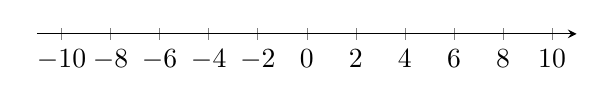
\begin{tikzpicture}
            \begin{axis}[
                xtick={-10,-8,...,10},
                axis x line=bottom, % only show the bottom x axis
                xmin=-11,
                xmax=11,
                hide y axis,
                ymin=0,
                ymax=1,
            ]
            \end{axis}
        \end{tikzpicture}
    \end{center}
    \end{example}
}
\frame{
		\frametitle{You Try 2:}
	\begin{alertblock}{You Try 2}
	Solve the inequality, graph the solution on the number line and write the solution in interval notation.
		$$n-\frac{1}{2}\leq \frac{7}{8}$$
		\vspace{2.5cm}
		\begin{center}
        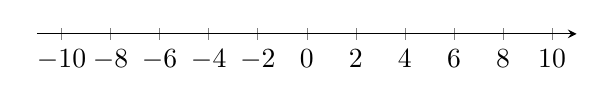
\begin{tikzpicture}
            \begin{axis}[
                xtick={-10,-8,...,10},
                axis x line=bottom, % only show the bottom x axis
                xmin=-11,
                xmax=11,
                hide y axis,
                ymin=0,
                ymax=1,
            ]
            \end{axis}
        \end{tikzpicture}
    \end{center}
    \end{alertblock}
}
\frame{
      \frametitle{Recall...}
    \begin{block}{Multiplication Property of Equality}
		\begin{align*}
		\text{If}&		&a&= b \\
		\text{Then}&	&ac&= bc
		\end{align*}
    \end{block}
	\begin{block}{Division Property of Equality}
		\begin{align*}
		\text{If}&		&a&= b \\
		\text{Then}&	&\frac{a}{c}&= b{c}
		\end{align*}
    \end{block}
}
\frame{
	  \frametitle{Positive $c$}
	\begin{block}{Let $c=5$}
		\begin{align*}
			Division&			&Multiplication \\
			10&< 15				&10&< 15
		\end{align*}
		\vspace{2.5cm}
	\end{block}
}
\frame{
	  \frametitle{Negative $c$}
	\begin{block}{Let $c=-5$}
		\begin{align*}
			Division&			&Multiplication \\
			10&< 15				&10&< 15
		\end{align*}
		\vspace{2.5cm}
	\end{block}
}
\frame{
	  \frametitle{The Takeaway}
	\begin{block}{Remember}
		When we divide or multiply an inequality by a:
		\begin{itemize}
			\item {\bf positive} number, the inequality stays the {\bf same}.
			\item {\bf negative} number, the inequality {\bf reverses}.
		\end{itemize}
	\end{block}
}
\frame{
	  \frametitle{We Try 3}
	\begin{example}
		Solve the inequality, graph the solution on the number line, and write the solution in interval notation.
		$$7y<42$$
		\vspace{2.5cm}
				\begin{center}
        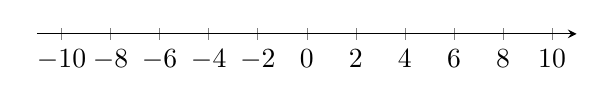
\begin{tikzpicture}
            \begin{axis}[
                xtick={-10,-8,...,10},
                axis x line=bottom, % only show the bottom x axis
                xmin=-11,
                xmax=11,
                hide y axis,
                ymin=0,
                ymax=1,
            ]
            \end{axis}
        \end{tikzpicture}
    \end{center}
	\end{example}
}
\frame{
	  \frametitle{You Try 3}
	\begin{alertblock}{You Try 3}
		Solve the inequality, graph the solution on the number line, and write the solution in interval notation.
		$$-7r\leq-70$$
		\vspace{2.5cm}
				\begin{center}
        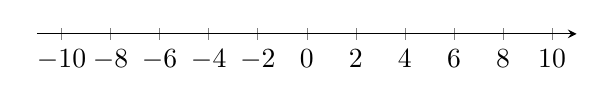
\begin{tikzpicture}
            \begin{axis}[
                xtick={-10,-8,...,10},
                axis x line=bottom, % only show the bottom x axis
                xmin=-11,
                xmax=11,
                hide y axis,
                ymin=0,
                ymax=1,
            ]
            \end{axis}
        \end{tikzpicture}
    \end{center}
	\end{alertblock}
}
\end{document}